%!TEX root = ../../thesis.tex
%*******************************************************************************
%****************************** Solution Implementation Chapter *********************************
%*******************************************************************************

\chapter{Solution Implementation}

\ifpdf
    \graphicspath{{Chapters/Implementation/Figs/}{Chapters/Implementation/Figs/}{Chapters/Implementation/Figs/}}
\else
    \graphicspath{{Chapters/Implementation/Figs/}{Chapters/Implementation/Figs/}}
\fi
In the previous chapter, we displayed an overview design of our approach.
Consequently, the solution implementation chapter of this thesis presents the details of how the proposed system was developed and implemented.
Firstly, we define some \ac{df} (see section \ref{implementation:section:designfeatures}) that focus on designing and developing new artifacts, methods, or systems.
Next, the description of the technology stack and development tools is explained (see section \ref{implementation:section:technologies}).
The chapter includes a detailed explanation of the critical features and functionality of the system and the processes used in frontend implementation (see section \ref{implementation:section:frontend}), database implementation (see section \ref{implementation:section:database}) backend implementation (see section \ref{implementation:section:backend}), and the software tool (see section \ref{implementation:section:tool}).
Through this chapter, readers will understand how we brought the proposed solution to reality and its potential for real-world applications.

\section{Tool Design Features (DFs)}
\label{implementation:section:designfeatures}
\ac{dsr} aims to produce a tangible outcome, such as a new software tool, a process improvement, or a theoretical framework.
It often involves multiple cycles of design, evaluation, and redesign, allowing for constant improvement of the artifact.
Since we perform the \textit{first} iteration of the cycle, we derive the features of our software tool using the \ac{df}s.
In this section, we translate each \ac{dp}s (we defined in chapter \ref{chap:design}) into a set of \ac{df}s that we can directly implement into the tool or solution approach and we describe the \ac{df}s for each of the derived \ac{dp}s.
As shown in the figure \ref{fig:implementation:hierarchy}, we see that the \ac{df}s are divided according to the \textit{LEAN} development cycle.
\clearpage

\begin{figure}[htbp!]
    \centering
    \begin{subfigure}[b]{1.0\textwidth}
    \centering
    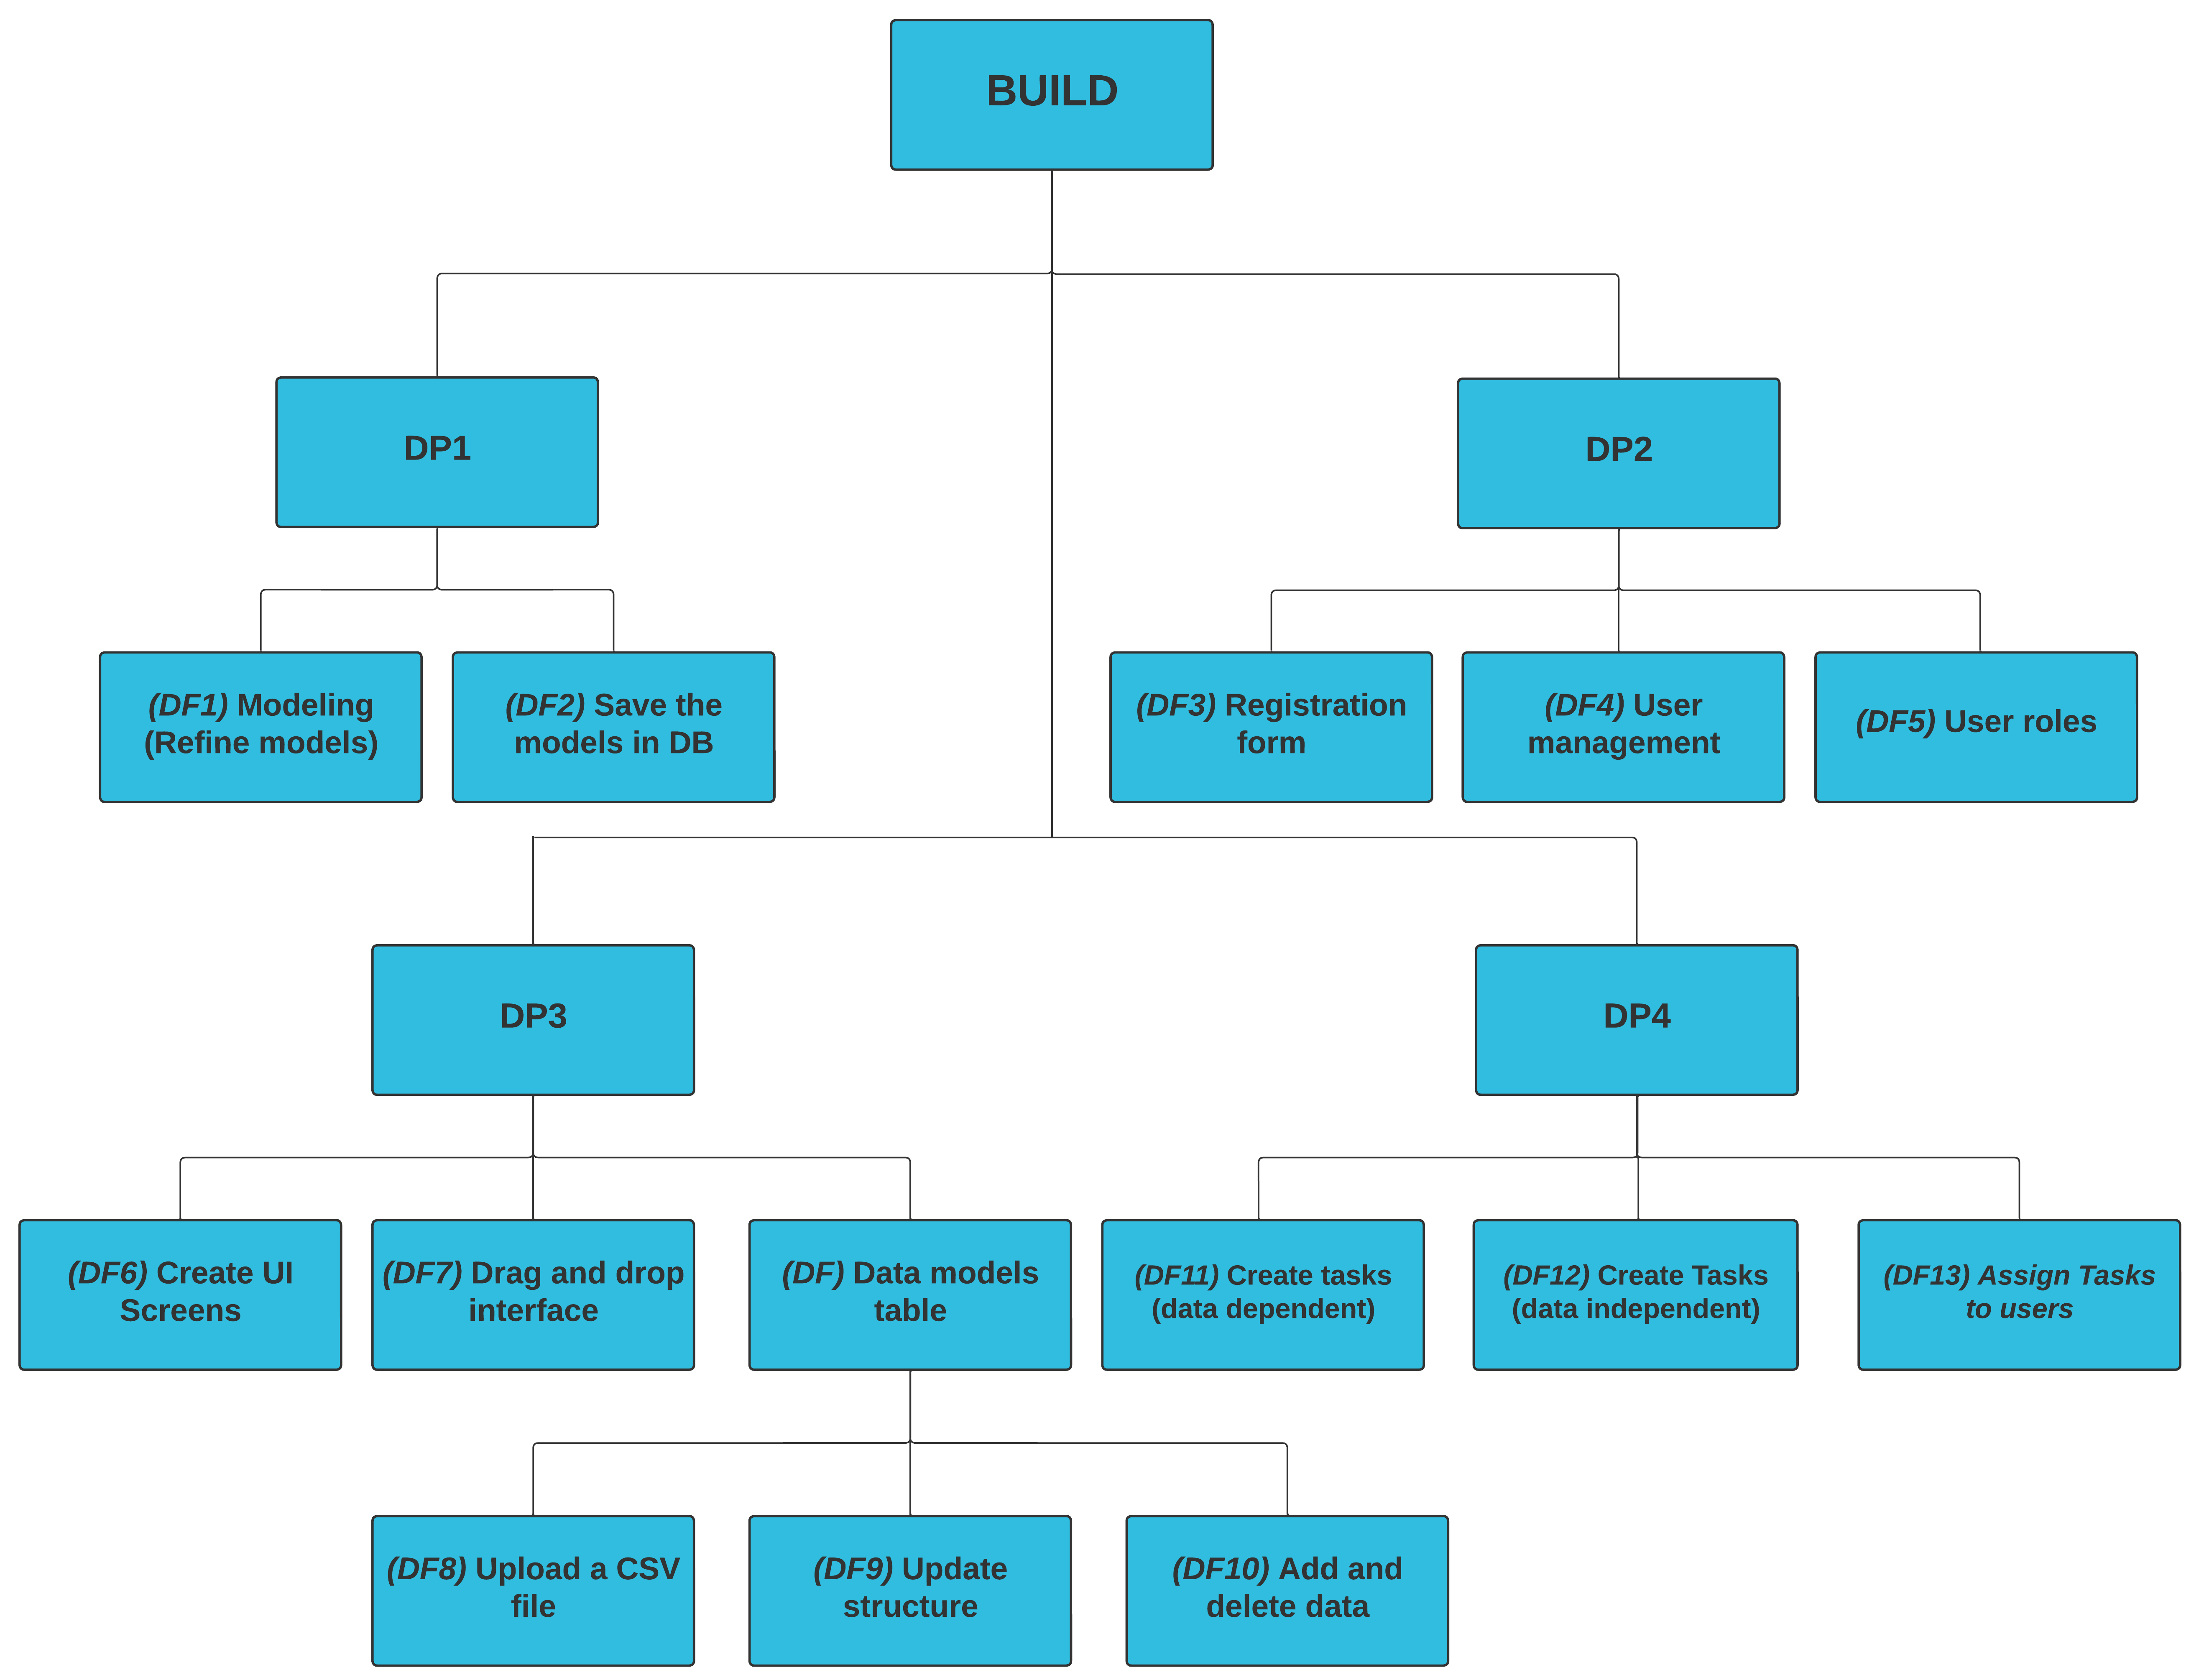
\includegraphics[width=0.8\textwidth]{DFs_hierarchy_build.png}
    \caption{A hierarchical diagram of \ac{df}s from \textit{Build} phase}
    \label{fig:implementation:hierarchy:build}
    \end{subfigure}
    \begin{subfigure}[b]{1.0\textwidth}
    \centering
    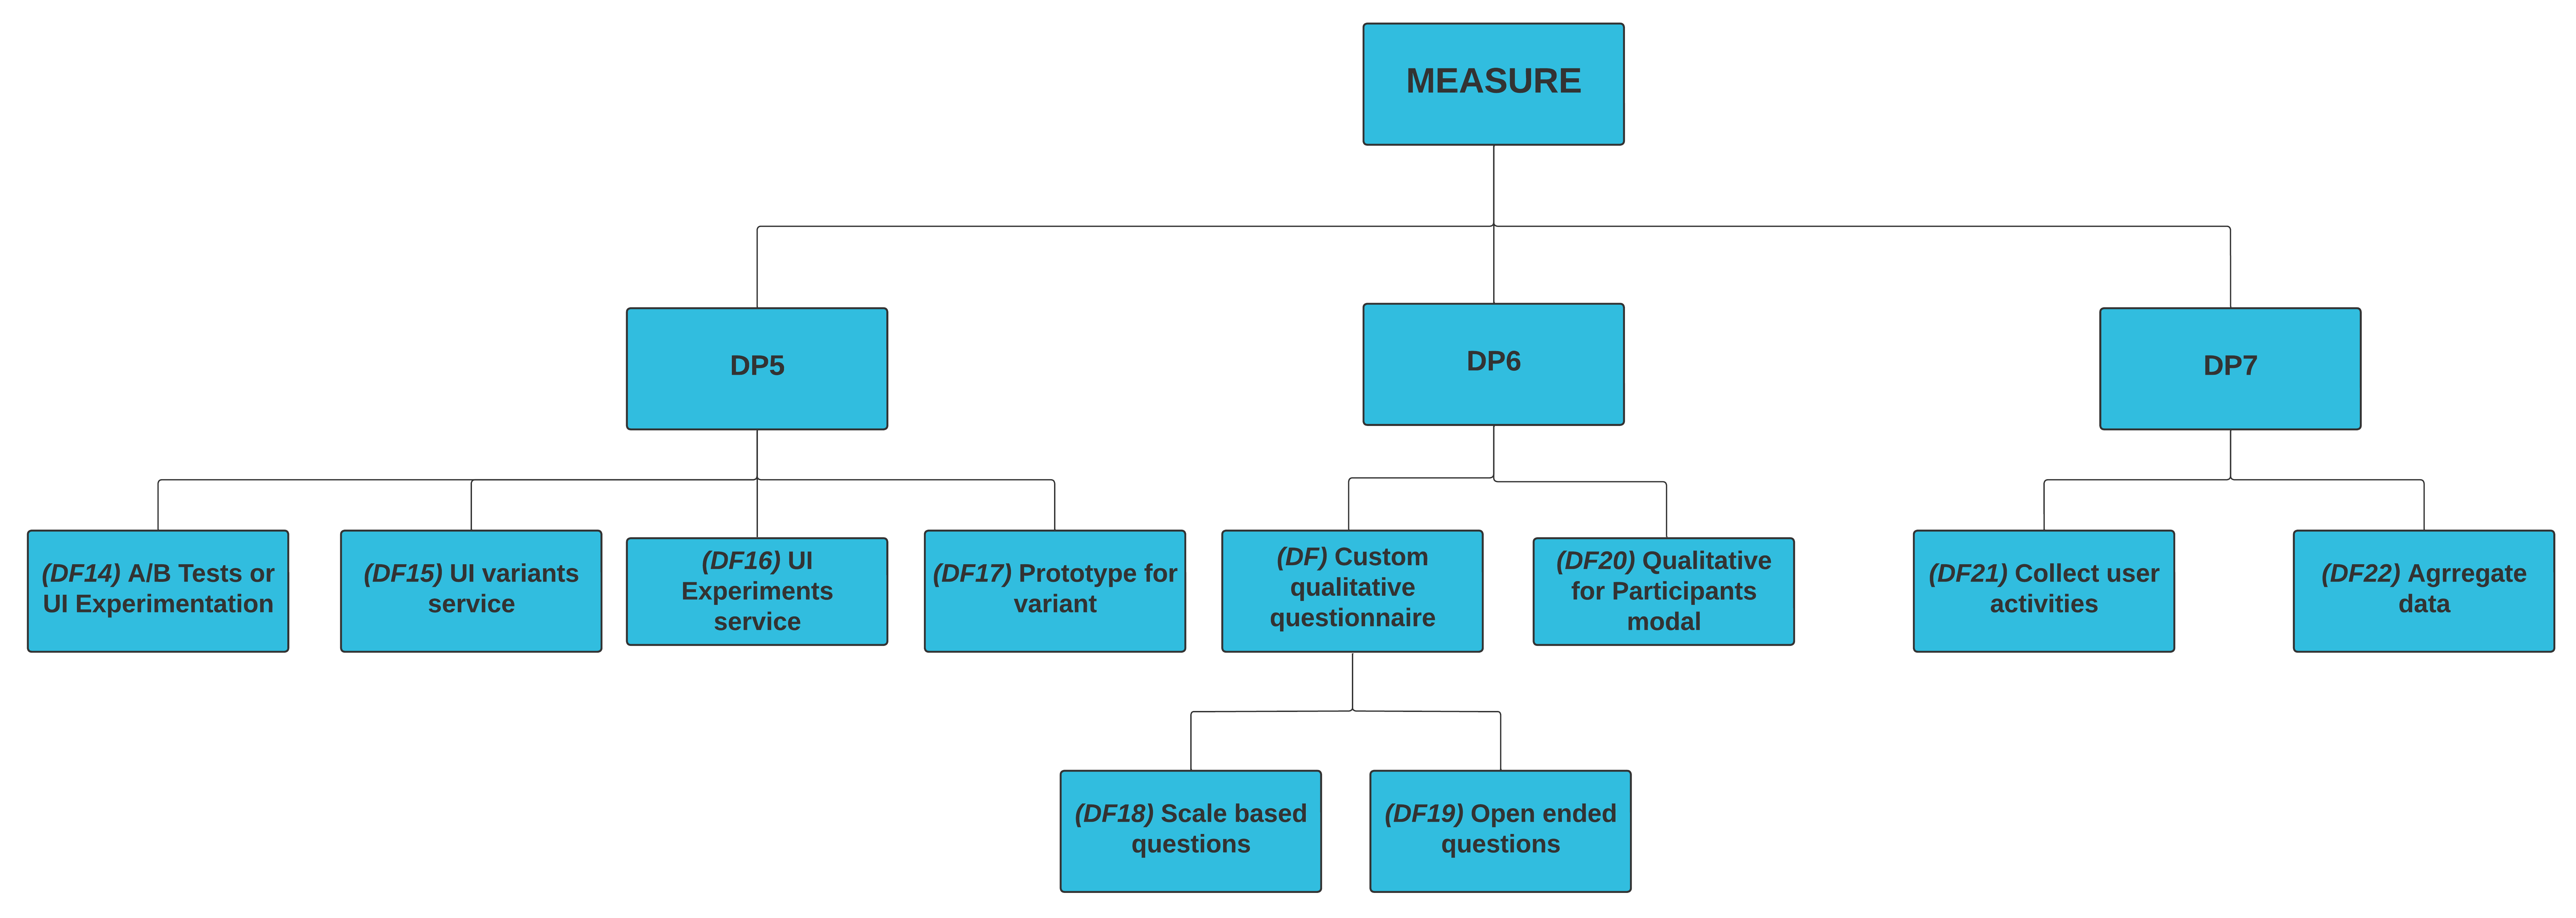
\includegraphics[width=1.1\textwidth]{DFs_hierarchy_measure.png}
    \caption{A hierarchical diagram of \ac{df}s from \textit{Measure} phase}
    \label{fig:implementation:hierarchy:measure} 
    \end{subfigure}             
    \begin{subfigure}[b]{0.8\textwidth}
    \centering
    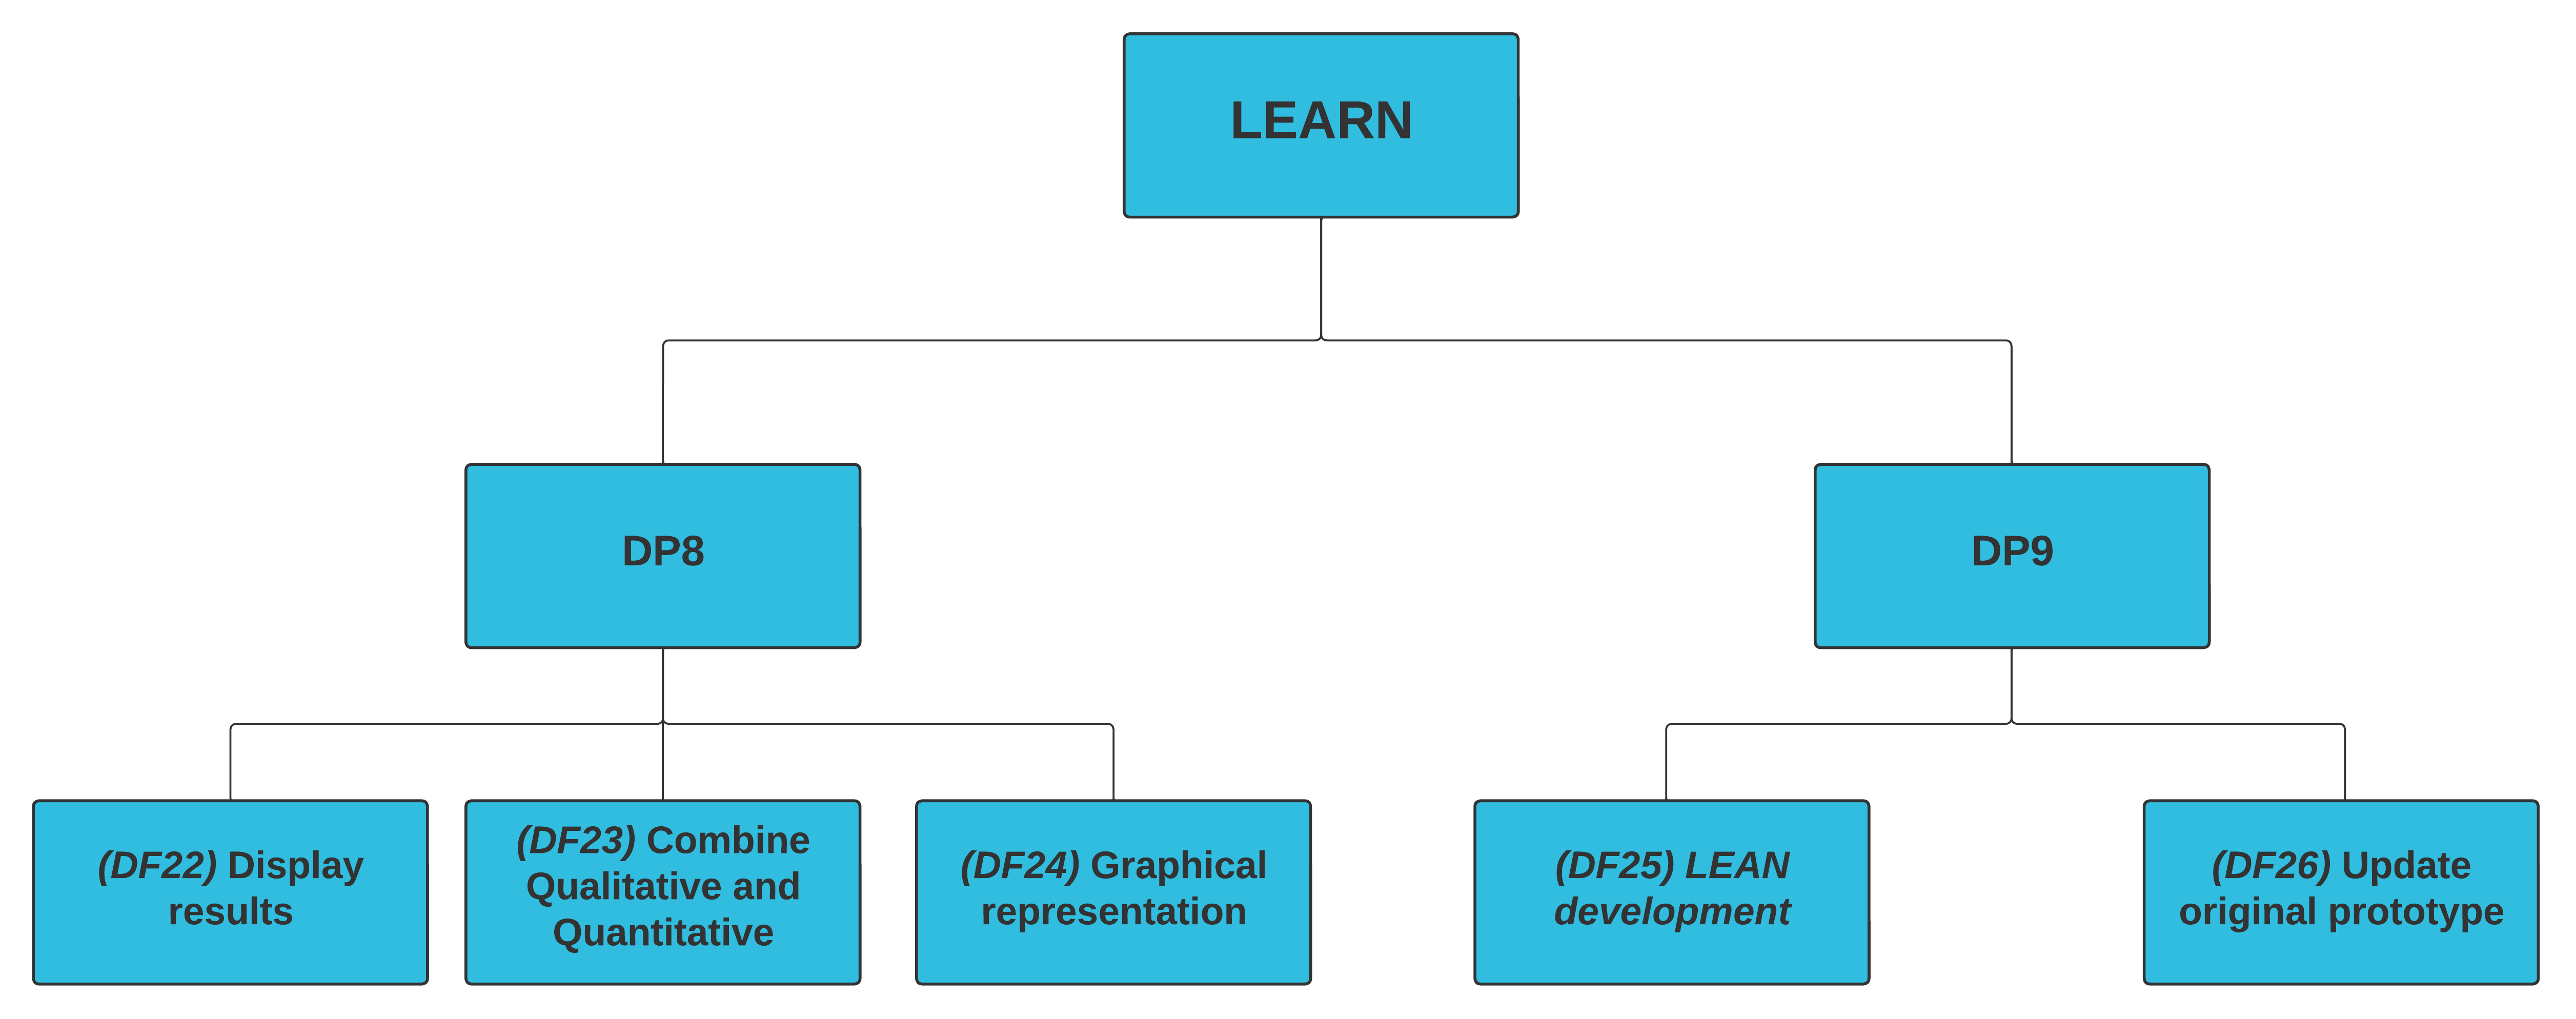
\includegraphics[width=1.0\textwidth]{DFs_hierarchy_learn.png}
    \caption{A hierarchical diagram of \ac{df}s from \textit{Learn} phase}
    \label{fig:implementation:hierarchy:learn}
    \end{subfigure}
    \caption[A map between \ac{dp}s and \ac{df}s]{Hierarchical structure of \ac{df}s}
    \label{fig:implementation:hierarchy}
\end{figure}
\paragraph{Build:}
In the \textit{Build} phase of the \textit{LEAN} development cycle, based on the \textbf{\ac{dp}1: Modeling}, the solution approach provides features for creating the models (\textit{\ac{df}1}) useful for persisting data in the database and updating them (\textit{\ac{df}2}) with the results of the experiments.
It helps to create our prototypes in a model-based approach and improve our prototypes by improving the models throughout the LEAN development cycle.
With the \textbf{\ac{dp}2: User Variety}, the key features of our solution approach for the \ac{ui} prototyping tool will include registration for diverse users using a registration form (\textit{\ac{df}3}) and user management, i.e., features that enable team members to create and manage user accounts (\textit{\ac{df}4}), assign different levels of access and permissions (\textit{\ac{df}5}).
The \textit{User module} maintains all these features and also the user authentication, authorization, and user profile management.
And then based on the \textbf{\ac{dp}3: Flexible UI Elements}, the privileged user prototypes using the features of our solution approach, which includes the creation of different screens (\textit{\ac{df}6}) and reusable \ac{ui} elements using a drag and drop interface (\textit{\ac{df}7}). 
The tool also provides a feature to add custom data i.e., creating data models by uploading a \ac{csv} file (\textit{\ac{df}8}), revising structures of data model table (\textit{\ac{df}9}), adding and deleting data from the table (\textit{\ac{df}10}).
Next, based on the \textbf{\ac{dp}4: User tasks Refinement}, the privileged user creates \textit{User Tasks} for the users using the features of our solution approach, which includes creating tasks for users depending on the data model (\textit{\ac{df}11}) and independent of data models (\textit{\ac{df}12}), and assign the task to the experiments (\textit{\ac{df}13}).

\paragraph{Measure:}
In the \textit{Measure} phase of the \textit{LEAN} development cycle, based on the \textbf{\ac{dp}5: Split Tests}, the privileged user would be able to create A/B tests or \ac{ui} experimentation (\textit{\ac{df}14}) using the features of our solution approach, which includes creating and modifying the experiments (\textit{\ac{df}15}), creating and updating the \ac{ui} variants (\textit{\ac{df}16}), and modifying the variants' prototypes such that each variant has a unique view (\textit{\ac{df}17}).
Next, based on the \textbf{\ac{dp}6: Qualitative Analysis}, the privileged user would be able to do qualitative analysis on the users using the features of our solution approach, which includes creating the custom qualitative questionnaire with options in the answering formats like \textit{Scale based}, i.e., the users will have to choose from options 1 to 10 (\textit{\ac{df}18}) and open-ended questions, i.e., the users will have the freedom to answer whatever they think (\textit{\ac{df}19}). 
And, the users will answer these questions after finishing the tasks with a modal appearing with different questions (\textit{\ac{df}20}). 
Similarly, based on the \textbf{\ac{dp}7: Quantitative Analysis}, the privileged user creates quantitative analysis on the users using the features of our solution approach, which includes collecting the task data feedback, i.e., collecting the time taken to finish the task, number of unsuccessful attempts, the path taken by the users to complete the task, etc. (\textit{\ac{df}21}), and aggregating these feedback data (\textit{\ac{df}22}). 

\paragraph{Learn:}
In the \textit{Learn} phase of the \textit{LEAN} development cycle, based on the \textbf{\ac{dp}8: Diversity in Analysis}, the privileged user compares the statistics using the features of our solution approach, which includes showing the results of the experiment (\textit{\ac{df}23}), combining qualitative and quantitative analysis of each variant (\textit{\ac{df}24}), and a graphical view to see the results (\textit{\ac{df}25}). 
Finally, based on the \textbf{\ac{dp}9: Continuous Design}, the solution approach would provide features including LEAN development cycle (\textit{\ac{df}26}). 
The privileged user should be able to update the original prototype with the results from the experiment (\textit{\ac{df}27}) for continuous improvement.

Overall, the design features section in DSR delivers a comprehensive overview of the solution tool to address the identified problem or research question. 
Moreover, this section describes the \ac{df}s for our \ac{poc} solution tool.
\clearpage

\section{Technologies Used}
\label{implementation:section:technologies}
We have created a software tool that allows us to test the features (\ac{df}s) and underlying principles of the developed DFs with actual users.
To test our solution approach, we developed a rapid prototyping tool for the first cycle of our \ac{dsr}. 

The implementation of our \textit{UI Prototyping Tool with Experimentation (UPTE)} platform uses various technologies.
Our UI prototyping tool was developed using Angular\footnote{A framework of javascript: \url{https://angular.io/}}, Loopback\footnote{A framework of the NodeJS \url{https://loopback.io/}}, and MongoDB\footnote{A non-relational database \url{https://www.mongodb.com/}}.
Angular is a JavaScript framework used for building web-based applications.
It provides comprehensive tools for creating dynamic and responsive UI components and handling user interactions.
With angular, we are using several other UI components which are available on Node package manager (npm)\footnote{NPM: \url{https://www.npmjs.com/}}.

Loopback is a Node.js\footnote{NodeJS: \url{https://nodejs.org/en/}} framework used for building RESTful APIs. 
It provides an intuitive interface for creating API endpoints and managing data persistence. 
Loopback's support for various data sources, including relational and NoSQL databases, makes it a versatile choice for web applications. 
We connect our database using the data managers provided by the loopback framework.
The framework's ability to generate API documentation and testing tools simplifies our development process.

MongoDB is a NoSQL document-oriented database used for storing unstructured data. 
We store our prototyping tool's data using a JSON\footnote{What is JSON: \url{https://developer.mozilla.org/en-US/docs/Glossary/JSON}} format in an unstructured manner.
It provides a scalable and flexible solution for managing volumes of data. 
MongoDB's support for automatic sharding and replication ensures high availability and fault tolerance. 
The database's dynamic schema and rich query language make it easy to adapt to changing data requirements.

By leveraging these technologies, our UI prototyping tool delivered a powerful and user-friendly interface while ensuring efficient data retrieval and storage.
Based on these technologies, we build a microservice architecture explained in the next section so that our \ac{dp}s and \ac{df}s can be easily implemented. 
\clearpage

% \section{Solution Architecture}
% \label{implementation:section:architecture}

\section{Frontend Implementation}
\label{implementation:section:frontend}

This section discusses the front-end implementation of our software tool. 
As discussed in the previous section, we developed the \ac{ui} using \textit{Angular}, a popular front-end framework. 
Angular provides a comprehensive architecture (see figure \ref{implementation:fig:angulararchitecture}\footnote{Fig taken from: \url{https://www.geeksforgeeks.org/angular-7-architecture/}}) that includes components, templates, event binding, property binding, directives, and injectors. 
Angular's architecture is organized into modules containing specific functions designed to achieve particular goals. 
These modules can be imported and exported between different Angular applications. 
In each application, a root module is launched at the start of the application and imports other modules to add additional functionality.

\begin{figure}[ht]
    \centering
    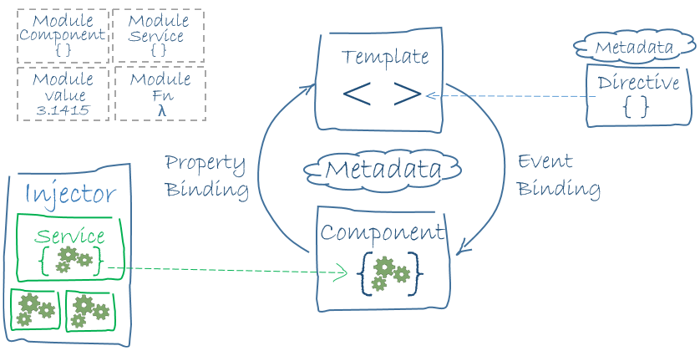
\includegraphics[scale=0.5]{angular-architecture.png}
    \caption[Angular Architecture]{Angular Architecture}
    \label{implementation:fig:angulararchitecture}
\end{figure}

In our implementation, the angular application has a root entry point, a module file (see Listing \ref{listing:implementation:allmodule}), containing all the necessary imports to function properly. 
Within our NgModule, we have imported various user-developed modules and third-party modules like \textit{MatInputModule}, \textit{NgxMatFileInputModule}, and \textit{DragDropModule} for UI elements. 
By importing these modules, we can utilize their functions and features within our application to enhance its overall functionality and user experience.
One key benefit of using \textit{Angular Material Design}\footnote{Website for Angular material design: \url{https://v7.material.angular.io/}} is providing a library of pre-built UI components that follow Material Design guidelines, such as buttons, forms, and navigation menus. 
It saves time designing and developing UI elements from scratch and instead focuses on customizing them to fit our needs.
\textit{Nginx File Input}\footnote{Website for Angular Material File Input \url{https://www.npmjs.com/package/@angular-material-components/file-input}} is another third-party module we have imported into our application. 
This module allows users to upload files directly from their local device, enabling us to save them to our server for future use.
Finally, the \textit{Drag and Drop module}\footnote{Website for the Angular material Drag and drop \url{https://v7.material.angular.io/cdk/drag-drop/api}} allows users to easily rearrange elements on the \ac{ui} by dragging and dropping them to their desired location. 
Utilizing this module can provide a more interactive and dynamic user experience for prototyping.

\begin{lstlisting}[language=JavaScript, caption=all-component.module.ts, label=listing:implementation:allmodule]
// Components
import { LoginComponent } from './components/login/login';
...
// Modules
import { DragDropModule } from '@angular/cdk/drag-drop';
import { AppRoutingModule } from '../app-routing.module';
import { NgxMatFileInputModule } from '@angular-material-components/file-input';
// Material design
import { MatSidenavModule } from '@angular/material/sidenav';
...

@NgModule({
    declarations: [
        LoginComponent,
        ...
    ],
    imports: [
        DragDropModule,
        AppRoutingModule,
        NgxMatFileInputModule,
        MatSidenavModule,
        ...
    ],
    exports: [
        LoginComponent, 
        ...
    ]
})
export class AllComponentModule { }  
\end{lstlisting}

Our implementation focuses on the \ac{mvc} architecture, which contains services and directives to talk to the server and some middleware to add a user token to every request to authenticate the user. In the next section, we explain how we implemented the \textit{UI Prototyping component}.
In our tool, we have implemented \textit{left-panel}, \textit{middle-panel}, and \textit{right-panel} components, dividing our screen. 
Then, we use the \textit{observer pattern}\footnote{Website for Observer pattern: \url{https://refactoring.guru/design-patterns/observer}} for the interaction between these components and various services to interact with the server.

\begin{lstlisting}[language=JavaScript, caption=left-panel.component.ts, label=listing:implementation:left]
import { NestedTreeControl } from '@angular/cdk/tree';
import { Component, OnInit } from '@angular/core';
...
@Component({
    templateUrl: './left-panel.component.html',
    ...
})
export class LeftPanelComponent implements OnInit {
    // Define variables ...
    constructor(private shared: CommunicationService, private viewService: ViewsService, ...) { }

    async ngOnInit() {
        // get master view from server
        let master: View = await firstValueFrom(this.viewService.getMasterView())
    }

    // CRUD of view
    addView(isMaster: boolean = false, node: View = new View()) {
        let master: View = this.dataSource.data[0]
        master.children.push(View.getView(false, name))
        this.dataSource = new MatTreeNestedDataSource<View>()
    }
    ...

    // Emit events and the other panels/components capture them
    addElement(elementName: string) {
        this.shared.setAddUIElement(elementName)
    }

}    
\end{lstlisting}
\paragraph{Left panel}
The left-panel component contains a list of UI elements that can be added to the screen.
It allows users to navigate and manipulate the elements on the screen easily, improving the \ac{ux}.
In our implementation (see Listing \ref{listing:implementation:left}), firstly, we added a \texttt{@Component} directive to the component's TypeScript file to specify the location of its template file, CSS file and selector.
Next, we added a function that fetches the master view, if present in the database, and assigns it to a variable in the component's code. 
This function is called during the initialization of the component called \texttt{ngOninit}. 
We also included functionality for CRUD operations for the views or UI screens in the prototyping phase. 
It includes adding, editing, deleting, and viewing views or UI screens. 
Finally, we had several functions that emit events to other panels or components that are listening to these events. 
It allows for communication and coordination between different parts of the application.
Similarly, the template of the left panel contains a tree structure that displays the views and their children. 
This structure allows users to easily navigate through different UI screens and select the one they want to work on. 
The left panel template also contains various UI elements that the user can add to the UI screen in the middle panel.
We have grouped them into different categories based on functionality, such as form elements, buttons, text elements, etc. 
Each category can be expanded or collapsed to make it easier to find the desired element.

\paragraph{Middle Panel}
In our implementation, firstly, in the constructor, the middle panel component (see Listing \ref{listing:implementation:middle}) creates a renderer to listen to mouse and keyboard events.
This component subscribes to the required events that are emitted by other components. 
For example, it listens to adding UI elements from the left panel component. 
After the event is subscribed it adds the required UI element to the screen using the \texttt{addUIElement()} method and the provided information.
It then uses the \textit{Drag API} to make the element draggable within the virtual screen and adds various listeners.
When the element is moved and placed at a certain position, the draggable interface provides the element's position, which is then added to the data structure of the current element.  
This component also provides CRUD functionality for the UI elements, i.e. to add, update, remove elements.
For instance, it adds listeners for the keyboard events, such as delete or backspace key press, and removes the element from the screen when the event is triggered.
Similarly, we implemented a template for the middle panel component that allows the user to build the prototype visually. 
The template is designed to provide a virtual screen for the user to place UI elements. 
It contains a box that defines the dimensions of the screen and displays the name of the current view that is being edited. 
The user can place UI elements within the box by dragging and dropping them onto the screen. 
These elements are provided by the left panel component and can be customized using the properties panel component on the right. 
The middle panel component subscribes to events emitted by the left and right panel components, allowing it to update the screen in real-time.

\begin{lstlisting}[language=JavaScript, caption=middle-panel.component.ts, label=listing:implementation:middle]
@Component({...})
export class MiddlePanelComponent implements OnInit {
    // Define variables
    @ViewChild('cardContent') el!: ElementRef
    ...
    constructor(private rf:RendererFactory2,private drag:DragDrop) {
        this.renderer = this.rf.createRenderer(null, null);
    }
    async ngOnInit() {
        // Subscribe to events e.g. add UI element
        await firstValueFrom(this.shared.getAddUIElement())
        this.addUIElement()
    }
    addUIElement() {
        // Define Component
        let component: ComponentContainer = new ComponentContainer()
        component.name = this.toAddElement
        ...
        // Make it draggable
        let dragRef: DragRef = this.drag.createDrag(recaptchaContainer).withBoundaryElement(this.el)
        // Add Element, push to array, add listener
        const text = this.renderer.createText(this.toAddElement)
        this.elementsOnCanVas.push(component)
        this.addListener(recaptchaContainer, component)
        this.getPosition(dragRef, component.id)
        ...
    }
    async getPosition(dragRef: DragRef, id: string) {
        const val = await firstValueFrom(dragRef.ended)
        toAdd.cssProperty.dropPoint = dragRef.getFreeDragPosition()
    }
    async addListener(elm: Element, el: ComponentContainer) {
        // Delete the element 
        const event = await this.renderer.listen(elm, 'keydown')
        if (event.key == 'Delete' || event.key == 'Backspace') {
            elm.remove() ...
        }
    }
}
\end{lstlisting}

\begin{lstlisting}[language=JavaScript, caption=right-panel.component.ts, label=listing:implementation:right]
@Component({...})
export class RightPanelComponent implements OnInit {
    // Define variables
    ...
    constructor(...) { }

    ngOnInit() {
        // Functions for subscribing to various events
        this.updateSelectedElement()
        this.getProperties()
        this.updateCanvasView()
        this.updateDeletionUIElement()
    }
    async updateCanvasView() {
        this.element = await firstValueFrom(this.shared.getCanvasView())
        this.elementName = val.name
        if (this.element.type == ContainerType.VIEW) {
            this.element.cssProperty = new CSSProperty().json
            this.element.cssProperty.height = '200'
        }
    }

    addNewInteraction() {
        const interaction: OnClickInteraction = new OnClickInteraction();
        interaction.id = uuidv4();
        this.element.interactions = [interaction]
    }
}    
\end{lstlisting}

\paragraph{Right Panel}
In our implementation, the right panel component serves as a property editor for the selected UI element in the middle panel. 
It contains various functions which are explained using the Listing \ref{listing:implementation:right}.
It listens to events emitted by the left panel and middle panel components to update the selected element's properties. 
It also listens to events to edit the canvas or screen and to delete the element from the canvas.
The right panel contains various input fields and dropdowns to edit the properties of the selected UI element, such as color, text, font, size, etc. 
When the user selects an element on the canvas, the right panel updates with the properties of that element. 
Similarly, when a new UI element is added to the canvas, the right panel displays the default properties for that element.
Additionally, the right panel contains a function for adding new interactions to the UI element, such as \texttt{onClick} event. 
This function allows the user to define a JavaScript function that will be executed when the UI element is clicked. 
The function can be added to the element's properties in the right panel and saved to the database along with the other properties.

\section{Backend Implementation}
\label{implementation:section:backend}

\section{Database Schema}
\label{implementation:section:database}


\section{Software Tool}
\label{implementation:section:tool}